
Monte Carlo Tree Search (MCTS), and especially UCT \cite{Kocsis.uct}
appears in numerous search applications, such
as \cite{Eyerich.ctp}. Although these methods are shown to be
successful empirically, most authors appear to be using UCT ``because
it has been shown to be successful in the past'', and ``because it
does a good job of trading off exploration and exploitation''. While
the latter statement may be correct for the Multi-armed Bandit problem (MAB)
and for the UCB1 algorithm \cite{Auer.ucb}, we argue that a simple
reconsideration from basic principles can result in schemes that
outperform UCT.

The core issue is that in MCTS for adversarial search and search in
``games against nature'' the goal is typically to find the best
first action of a good (or even optimal) policy, which is closer to
minimizing the simple regret, rather than the cumulative regret
minimized by UCB1.  However, the simple and the cumulative regret
cannot be minimized simultaneously; moreover, \cite{Bubeck.pure} shows
that in many cases the smaller the cumulative regret, the greater the
simple regret.

We begin with background definitions and related work.  VOI estimates
for arm pulls in MAB are presented, and a VOI-aware sampling policy is
suggested, both for the simple regret in MAB and for MCTS.  Finally,
the performance of the proposed sampling policy is evaluated on sets
of Bernoulli arms and on Computer GO, showing the improved
performance.

\section{Background and Related Work}
\label{sec:mcts-related-work}

Monte-Carlo tree search was initially suggested as a scheme for
finding approximately optimal policies for Markov Decision Processes
(MDP).  MCTS explores an MDP by performing
\emph{rollouts}---trajectories from the current state to a state in
which a termination condition is satisfied (either the goal or a
cutoff state).

Taking a sequence of samples in order to minimize the regret of a
decision based on the samples is captured by the Multi-armed Bandit
problem (MAB) \cite{Vermorel.bandits}. In MAB, we have a set of $K$
arms. Each arm can be pulled multiple times. When the $i$th arm is
pulled, a random reward $X_i$ from an unknown stationary distribution
is encountered. In the \textit{cumulative setting}, all encountered rewards are
collected.  UCB1 \cite{Auer.ucb} was shown to be
near-optimal in this respect. UCT, an extension of UCB1 to MCTS is
described in \cite{Kocsis.uct}, and shown to outperform many state of
the art search algorithms in both MDP and adversarial search
\cite{Gelly.mogo,Eyerich.ctp}. In the \textit{simple regret setting}, the agent
gets to collect only the reward of the last pull.
\begin{dfn}
The \textbf{simple regret} of a sampling policy for MAB
is the expected difference between the best expected reward
$\mu_*$ and the expected reward $\mu_j$ of the empirically best arm
$\overline X_j=\max_i\overline X_i$:
\begin{equation}
\IE r=\sum_{j=1}^K\Delta_j\Pr(\overline X_j=\max_i\overline X_i)
\label{eqn:mcts-simple-regret}
\end{equation}
where $\Delta_j=\mu_*-\mu_j$.
\end{dfn}
Strategies that minimize the simple regret are called pure exploration
strategies \cite{Bubeck.pure}. 

A different scheme for control of sampling can use the principles of 
rational metareasoning (Section~\ref{sec:ratimeta}).
In particular, a pure exploration strategy  based on the principles of
rational metareasoning would always select a sample with the highest
value of information, and stop the sampling when the VOI of the sample
is lower than the cost.

\section{Upper bounds on Value of Information}
\label{sec:mcts-approx-nonbayesian-section}

In many practical applications of the selection problem, such as search in
the game of Go, prior distributions are unavailable.\footnote{The analysis is also applicable to
some Bayesian settings, using ``fake" samples to simulate prior distributions.}
In such cases, one can still bound
the value of information of myopic policies using {\em concentration
inequalities} to derive distribution-independent bounds on the
VOI. We obtain such bounds under the
following assumptions:
\begin{enumerate}
\item Samples are iid given the value of the arms (variables), as in the Bayesian schemes such as Bernoulli
sampling.
\item The expectation of a selection in a belief state is equal to the sample mean (and therefore,
   after sampling terminates, the arm with the greatest sample mean will be selected).
\end{enumerate}

When considering possible samples in the blinkered semi-myopic setting,
two cases are possible: either
	the arm $\alpha$ with the highest sample mean $\overline
  	X_\alpha$ is tested, and $\overline X_\alpha$ becomes lower than
 	$\overline X_\beta$ of the second-best arm $\beta$;
or, 
	another arm~$i$ is tested, and $\overline X_i$ becomes higher
    than $\overline X_\alpha$.


Our bounds below are applicable to any bounded distribution (without loss of generality 
bounded in $[0,1]$). Similar
bounds can be derived for certain unbounded distributions, such as the
normally distributed prior value with normally distributed
sampling.
We derive a VOI bound for testing an arm a fixed $N$ times,
where $N$ can be the remaining budget of available samples or
any other integer quantity.
Denote by  $\Lambda_i^b$ the intrinsic VOI of testing the $i$th arm
$N$ times, and the number of
samples already taken from the $i$th arm by $n_i$.
\begin{thm} $\Lambda_i^b$ is bounded from above as
\begin{align}
\label{eqn:mcts-thm-be}
\Lambda_{i|i\ne\alpha}^b&\le \frac {N(1-\overline X_\alpha^{n_\alpha})} {n_i}\Pr(\overline   X_i^{{n_i}+N}\ge\overline X_\alpha^{n_\alpha})\nonumber\\
\Lambda_\alpha^b&\le \frac {N \overline X_\beta^{n_\beta}} {n_\alpha} \Pr(\overline X_\alpha^{n_\alpha+N}\le\overline X_\beta^{n_\beta})
\end{align}
\label{thm:mcts-be}
\end{thm}
\begin{proof} For the case $i\ne \alpha$, the probability that the
	  $i$th arm is finally chosen instead of $\alpha$ is
	  $\Pr(\overline X_i^{n_i+N} \ge \overline X_\alpha^{n_\alpha})$. $X_i \le 1$,
	  therefore $\overline X_i^{n_i+N}\le \overline
	  X_\alpha^{n_\alpha}+\frac {N(1-\overline X_\alpha^{n_\alpha})} {N+n_i}$. Hence, the intrinsic value of blinkered
	  information is at most: 
	\begin{align}
	\label{eq:simplistic}
	\frac{ N(1-\overline  X_\alpha^{n_\alpha})}
	  {N+n_i}&\Pr(\overline X_i^{{n_i}+N}\ge\overline X_\alpha^{n_\alpha})\nonumber \\
	&\le\frac{ N(1-\overline  X_\alpha^{n_\alpha})}
	{n_i}\Pr(\overline X_i^{{n_i}+N}\ge\overline X_\alpha^{n_\alpha})
	\end{align}
	  Proof for the case $i=\alpha$ is similar.
\end{proof}


The probabilities can be bounded from above using the
Hoeffding inequality \cite{Hoeffding.ineq}:
\begin{thm} For any $A\ge\overline X_{i|i\ne\alpha}^{n_i}$ and $B\le\overline X_\alpha^{n_\alpha}$ the probabilities $\Pr(\overline X_{i|i\ne\alpha}^{n_i+N} \ge A)$, $\Pr(\overline X_\alpha^{{n_\alpha}+N} \le B)$ are bounded from above as
\begin{align}
  \label{eqn:mcts-probound-blnk-hoeffding}
  \Pr&(\overline X_{i|i\ne\alpha}^{n_i+N} \ge A) \le 2\exp\left(- \varphi (A -\overline  X_i^{n_i})^2 n_i \right)\nonumber\\
  \Pr&(\overline X_\alpha^{{n_\alpha}+N} \le B) \le 2\exp\left(- \varphi (\overline X_\alpha^{n_\alpha} - B)^2 n_\alpha\right)
\end{align}
where $\varphi=\min \left(2(\frac {1+n/N} {1+\sqrt {n/N}})^2\right)=8(\sqrt 2 - 1)^2 > 1.37$.
\label{thm:mcts-hoeffding-prob-bounds}
\end{thm}


\begin{proof}
	Equation~(\ref{eqn:mcts-probound-blnk-hoeffding}) follows from
        the observation that $\overline X_i^{n_i+N}>A$ if and only if
        the mean $\overline X_i^N$ of $N$ samples from $n_i+1$ to
        $n_i+N$ is at least $A+(A-\overline X_i^{n_i})\frac {n_i} N$.

	For any $\delta$, the probability that $\overline X_i^{n_i+N}$ is greater
	than $A$ is less than the probability that
	$\IE[X_i]\ge\overline X_i^n+\delta$
	\emph{or} $\overline X_i^N\ge \IE[X_i]+A -\overline X_i^{n_i} - \delta +(A - \overline X_i^{n_i})\frac {n_i} N$,
	thus, by the union bound, less than the sum of the probabilities:
	\begin{align}
	\Pr&(\overline X_i^{n_i+N}\ge A)\nonumber\\
	   &\le\Pr(\IE[X_i]-\overline X_i^{n_i} \ge \delta)\\
	   &+\Pr\left(\overline X_i^N - \IE[X_i] \ge A
	           - \overline X_i^{n_i} - \delta +(A - \overline X_i^{n_i})\frac {n_i} N\right)\nonumber
	\end{align}
	Bounding the probabilities on the right-hand side using the Hoeffding
	inequality, obtain:
	\begin{align}
	\Pr&(\overline X_i^{n_i+N}\ge A)\nonumber\\
	    &\le\exp(-2\delta^2n_i)\nonumber\\
	    &+\exp\left(-2\left((A - \overline X_i^{n_i})\left(1+\frac {n_i} N\right)-\delta\right)^2N\right)
	\label{eqn:mcts-app-hoeffding-le-maxexp}
	\end{align}
	Find $\delta$ for which the two terms on the right-hand side of
	Equation~(\ref{eqn:mcts-app-hoeffding-le-maxexp}) are equal:
	\begin{equation}
	\exp(-\delta^2n) = \exp\left(-2\left((A - \overline X_i^{n_i})(1+\frac {n_i} N) - \delta\right)^2N\right)\label{eqn:mcts-app-hoeffding-eq-exp}
	\end{equation}
	Solve Equation~(\ref{eqn:mcts-app-hoeffding-eq-exp}) for $\delta$: $\delta=\frac {1+\frac {n_i} N} {1+\sqrt {\frac {n_i} N}} (A - \overline X_i^{n_i}) \ge 2(\sqrt 2 - 1)(A-\overline X_i^{n_i})$. Substitute $\delta$ into 
	Equation~(\ref{eqn:mcts-app-hoeffding-le-maxexp}) and obtain
	\begin{align}
	\Pr&(\overline X_i^{n_i+N}\ge A) \nonumber\\
	& \le 2\exp\left(-2\left( \frac {1+\frac {n_i} N} {1+\sqrt {\frac {n_i} N}}
	                          (\overline X_\alpha^{n_\alpha} - \overline X_i^{n_i})\right)^2 n_i\right)\nonumber \\
	& \le 2\exp(-8(\sqrt 2 - 1)^2(A - \overline X_i^{n_i})^2n_i)\nonumber\\
	& = 2\exp(-\varphi(A - \overline X_i^{n_i})^2n_i)
	\end{align}
	Derivation for the case $i=\alpha$ is similar.
\end{proof}	

\begin{crl}
An upper bound on the VOI estimate $\Lambda_i^b$ is obtained
by substituting Equation~(\ref{eqn:mcts-probound-blnk-hoeffding}) into (\ref{eqn:mcts-thm-be}).
\begin{align}
  \label{eqn:mcts-bound-blnk-hoeffding}
  \Lambda&_{i|i\ne\alpha}^b\le \hat\Lambda_i^b=  \frac {2N(1-\overline  X_\alpha^{n_\alpha})} {n_i}\exp\left(- \varphi(\overline X_\alpha^{n_\alpha} - \overline X_i^{n_i})^2 n_i\right)\\
  \Lambda&_\alpha^b \le \hat\Lambda_\alpha^b=\frac {2N\overline X_\beta^{n_\beta}} {n_\alpha}\exp\left(- \varphi(\overline X_\alpha^{n_\alpha} - \overline X_\beta^{n_\beta})^2 n_\alpha\right)\nonumber
\end{align}
\label{crl:bound-blnk-hoeffding}
\end{crl}

More refined bounds can be obtained through tighter estimates on the
probabilities in Equation~(\ref{eqn:mcts-thm-be}), for example, based on the empirical Bernstein
inequality~\cite{MaurerPontil.benrstein}, or through a more careful
application of the Hoeffding inequality, resulting in Theorem~\ref{thm:mcts-better-bound-blnk-hoeffding}:
\begin{thm} $\Lambda_i^b$ is bounded from above as
\begin{align}
\Lambda_{i|i\ne \alpha}^b&\le\frac {\sqrt \pi} {\sqrt {\varphi n_i}}
  \left[\mathrm{erf}\left(\left(\overline X_\alpha^{n_\alpha}+\frac N {N+n_i}(1-\overline X_\alpha^{n_\alpha})-\overline X_i^{n_i}\right)\sqrt {\varphi n_i}\right)
      -\mathrm{erf}\left((\overline X_\alpha - \overline X_i^{n_i})\sqrt{\varphi n_i}\right)\right]\nonumber\\
\Lambda_\alpha^b&\le\frac {\sqrt \pi} {\sqrt {\varphi n_\alpha}}
  \left[\mathrm{erf}\left(\left(\overline X_\alpha^{n_\alpha}-\overline X_\beta^{n_\beta}+\frac N {N+n_\alpha} \overline X_\beta^{n_\beta}\right)\sqrt {\varphi n_\alpha}\right)
      -\mathrm{erf}\left((\overline X_\alpha^{n_\alpha} - \overline X_\beta^{n_\beta})\sqrt{\varphi n_\alpha}\right)\right]
\label{eqn:mcts-erf-blinkered}
\end{align}
\label{thm:mcts-better-bound-blnk-hoeffding}
\end{thm}

\begin{proof}By definition,
\begin{equation}
\Lambda_i^b=\int\limits_{\overline X_\alpha}^{\overline X_\alpha^{n_\alpha}+\frac N {N+n_i}(1-\overline X_\alpha^{n_\alpha})}(x-\overline X_\alpha^{n_\alpha})\Pr\left(\overline X_i^{n_i+N}=x\right)dx
\label{eqn:mcts-lambda-blinkered-by-def}
\end{equation}
Integrating by parts, obtain
\begin{align}
\Lambda_i^b=&-\left.(x-\overline X_\alpha^{n_\alpha})\Pr\left(\overline X_i^{n_i+N}\ge x\right)\right|_{\overline X_\alpha^{n_\alpha}}^{\overline X_\alpha^{n_\alpha}+\frac N {N+n_i}(1-\overline X_\alpha^{n_\alpha})}+\int\limits_{\overline X_\alpha}^{\overline X_\alpha^{n_\alpha}+\frac N {N+n_i}(1-\overline X_\alpha^{n_\alpha})}\Pr\left(\overline X_i^{n_i+N}\ge x\right)dx\nonumber\\
=&\int\limits_{\overline X_\alpha}^{\overline X_\alpha^{n_\alpha}+\frac N {N+n_i}(1-\overline X_\alpha^{n_\alpha})}\Pr\left(\overline X_i^{n_i+N}\ge x\right)dx
\label{eqn:mcts-better-bound-by-parts}
\end{align}
Substituting the bound on $\Pr\left(\overline X_i^{n_i+N}\ge x\right)$ from Theorem~\ref{thm:mcts-hoeffding-prob-bounds} into (\ref{eqn:mcts-better-bound-by-parts}), finally obtain:
\begin{align}
\Lambda_i^b\le&\int\limits_{\overline X_\alpha}^{\overline X_\alpha^{n_\alpha}+\frac N {N+n_i}(1-\overline X_\alpha^{n_\alpha})}2\exp\left(-\varphi(x-\overline X_i^{n_i})^2n_i\right)dx\nonumber\\
 =&\frac {\sqrt \pi} {\sqrt {\varphi n_i}}
  \left[\mathrm{erf}\left(\left(\overline X_\alpha^{n_\alpha}+\frac N {N+n_i}(1-\overline X_\alpha^{n_\alpha})-\overline X_i^{n_i}\right)\sqrt {\varphi n_i}\right)-\mathrm{erf}\left((\overline X_\alpha - \overline X_i^{n_i})\sqrt{\varphi n_i}\right)\right]
\end{align}
Derivation for the case $i=\alpha$ is similar.
\end{proof}
\vspace{\baselineskip}
It is important to note that Corollary~\ref{crl:bound-blnk-hoeffding}
and Theorem~\ref{thm:mcts-better-bound-blnk-hoeffding}
provide actual bounds, rather than ``in probability''.

Selection problems usually separate out the decision of (1) {\em what}
to sample and (2) {\em whether} to sample or to stop (called the stopping criterion).
In this section we will examine the first issue, along with the empirical evaluation 
of the above approximate algorithms. The second issue --- the stopping
criterion --- is important in the context of sampling in trees, when the
selection problem is solved multiple times, at every node along the
path. This issue is explored in Section~\ref{sec:mcts-sampling-in-trees}.

Assuming that the sample costs are constant,
a semi-myopic policy will decide to test the arm that has the best
current VOI estimate. 
When the distributions are unknown, it makes sense
to use the upper bounds established in Theorem~\ref{thm:mcts-be}, as
we do in what follows. This evaluation assumes a fixed budget of samples, which is
completely used up by each of the candidate schemes, making a stopping
criterion irrelevant.

\begin{figure}[h!]
\centering
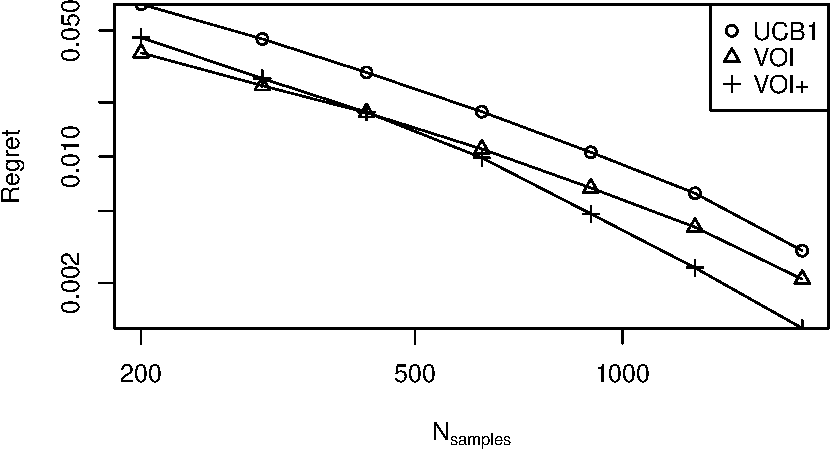
\includegraphics[scale=0.55]{mcts-flat.pdf}
\caption{Average regret of various policies as a function of the fixed number 
of samples in a 25-action Bernoulli sampling problem, over 10000 trials.}
\label{fig:random-instances}
\end{figure}

The sampling policies are compared on random Bernoulli
selection problem instances. Figure~\ref{fig:random-instances} shows results for
randomly-generated selection problems with 25 Bernoulli arms, where
the mean rewards of the arms are distributed uniformly in~$[0,1]$, 
for a range of sample budgets~$200..2000$, with multiplicative
step of~$2$, averaging over 10000 trials.  We compare UCB1 with the 
policies based on the bounds in
Equation~(\ref{eqn:mcts-bound-blnk-hoeffding}) (VOI) and
Equation~(\ref{eqn:mcts-erf-blinkered}) (VOI+).
UCB1 is always considerably worse than the VOI-aware sampling policies.


\section{Sampling in trees}
\label{sec:mcts-sampling-in-trees}

The previous section addressed the selection problem in the flat case.
Selection in trees is more complicated.  The goal of Monte-Carlo tree 
search \cite{Chaslot.montecarlo} at the root node 
is usually to select an action that appears to be the best based on outcomes
of \textit{search rollouts}.
But the goal of rollouts at non-root nodes
is different than at the root: here it is important to better approximate the
value of the node, so that selection at the root can be more informed. The exact analysis
of sampling at internal nodes is outside the scope of this study. At present we 
have no better proposal for internal nodes than to use UCT there.

We thus propose the following hybrid sampling scheme \cite{TolpinShimony.mcts}: 
	at the \emph{root node}, sample based on the VOI estimate;
	at \emph{non-root nodes}, sample using UCT.

Strictly speaking, even at the root node the stationarity assumptions
underlying our belief-state MDP for selection do not hold exactly. UCT
is an adaptive scheme, and therefore the values generated by sampling
at non-root nodes will typically cause values observed at children of
the root node to be non-stationary.  Nevertheless, sampling based on
VOI estimates computed as for stationary distributions works well in
practice. As illustrated by the empirical evaluation
(Section~\ref{sec:mcts-emp-go}), estimates based on
upper bounds on the VOI result in good sampling policies, which
exhibit performance comparable to the performance of some
state-of-the-art heuristic algorithms.


\subsection{Stopping criterion}
\label{sec:mcts-control-stopping-criterion}

When a sample has a known cost commensurable with the value of
information of a measurement, an upper bound on the intrinsic VOI can also
be used to stop the sampling if the intrinsic VOI of any arm
is less than the total cost of sampling $C$: $\max_i \Lambda_i \le C$.

The VOI estimates of Equations~(\ref{eqn:mcts-thm-be}) and~(\ref{eqn:mcts-bound-blnk-hoeffding})
include the remaining sample budget $N$ as a
factor, but given the cost of a single sample $c$, the cost of the
remaining samples accounted for in estimating the intrinsic VOI is
$C=cN$. $N$ can be dropped on both sides of the inequality,
giving a reasonable stopping criterion:
\begin{align}
\frac 1 N \Lambda_\alpha^b \le&\frac {\overline X_\beta^{n_\beta}}
  {n_\alpha}\Pr(\overline X_\alpha^{n_\alpha+N}\le\overline
  X_\beta^{n_\alpha})\le c\nonumber\\
\frac 1 N \max_i\Lambda_i^b\le &\max_i\frac {(1-\overline X_\alpha^{n_\alpha})} {n_i}\Pr(\overline
  X_i^{n_i+N}\ge\overline X_\alpha^{n_\alpha})\le c\nonumber\\
    &\forall i: i\ne\alpha
\label{eqn:mcts-stopping-blnk}
\end{align}
The empirical evaluation (Section~\ref{sec:mcts-emp-go})
confirms the viability of this stopping criterion and illustrates the
influence of the sample cost $c$ on the performance of
the sampling policy. When the sample cost $c$ is unknown, one can perform initial calibration experiments
to determine a reasonable value, as done in the following.

\subsection{Sample redistribution in trees}
\label{sec:mcts-control-redistribution}

The above hybrid approach assumes
that the information obtained from rollouts in the
current state is discarded after an real-world action is selected. In practice,
many successful Monte-Carlo tree search algorithms reuse rollouts
generated at earlier search states, if the sample traverses the
current search state during the rollout; thus, the value of information of a rollout is
determined not just by the influence on the choice of the action at
the current state, but also by its potential influence on the choice at future
search states.

One way to account for this reuse would be to incorporate the
`future' value of information into a VOI estimate. However, this 
approach requires a nontrivial extension of the theory of metareasoning for search.
Alternately, one can behave myopically with respect to the search tree depth:
\begin{enumerate}
\item Estimate VOI as though the information is discarded after each step,
\item Stop early if the VOI is below a certain threshold
   (see Section~\ref{sec:mcts-control-stopping-criterion}), and
\item Save the unused sample budget for search in future states, such that
   if the nominal budget is $N$, and the unused budget in the last state
   is $N_u$, the search budget in the next state will be $N+N_u$.
\end{enumerate}
In this approach, the cost $c$ of a sample in the current state is the
VOI of increasing the budget of a future state by one sample.  It is
unclear whether this cost can be accurately estimated, but supposing
a fixed value for a given problem type and algorithm implementation
would work. Indeed, the empirical evaluation (Section~\ref{sec:mcts-emp-go})
confirms that stopping and sample redistribution based on a learned
fixed cost  substantially improve the performance of the VOI-based
sampling policy in game tree search.


\subsection{Playing Go against UCT}
\label{sec:mcts-emp-go}

The hybrid policies were compared on the game Go, a search domain
in which UCT-based MCTS has been particularly successful
\cite{Gelly.mogo}. A modified version of Pachi \cite{Braudis.pachi}, a state of the art
Go program, was used for the experiments:
\begin{itemize}
\item The UCT engine of Pachi was extended with VOI-aware sampling
  policies at the first step. 
\item The stopping criterion for the VOI-aware policy was
  modified and based solely on the sample cost, specified as
  a constant parameter. The heuristic stopping criterion for the
  original UCT policy was left unchanged.
\item The time-allocation model based on the fixed number of samples
  was modified for \textit{both the original UCT policy and the VOI-aware
  policies} such that 
  \begin{itemize}
    \item Initially, the same number of samples is available to
      the agent at each step, independently of the number of pre-simulated
      games;  
    \item If samples were unused at the current step,
      they become available at the next step. 
  \end{itemize}
\end{itemize}
While the UCT engine is not the most powerful engine of Pachi, it is still a strong
player. On the other hand, additional features of more advanced
engines would obstruct the MCTS phenomena which are the subject of
the experiment.
\begin{figure}[h!]
\centering
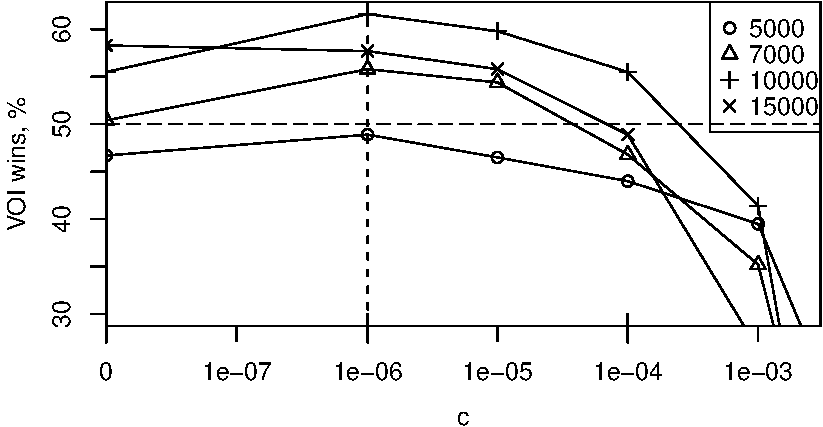
\includegraphics[scale=0.55]{mcts-uctvoi.pdf}
\caption{Winning rate of the VOI-aware policy in Go as a function of the cost $c$, for varying numbers of samples per ply.}
\label{fig:uctvoi}
\end{figure}
The engines were compared on the 9x9 board, for 5000, 7000, 1000, and
15000 samples (game simulations) per ply, each experiment repeated
1000 times. Figure~\ref{fig:uctvoi} depicts a calibration experiment,
showing the winning rate of the VOI-aware policy against UCT as a function of
the stopping threshold $c$ (if the maximum VOI of a sample is below
the threshold, the simulation is stopped, and a move is chosen). Each
curve in the figure corresponds to a certain number of samples per
ply.  For the stopping threshold of $10^{-6}$, the VOI-aware policy
is almost always better than UCT, and reaches the winning rate of
64\% for 10000 samples per ply.

\begin{figure}[h!]
\centering
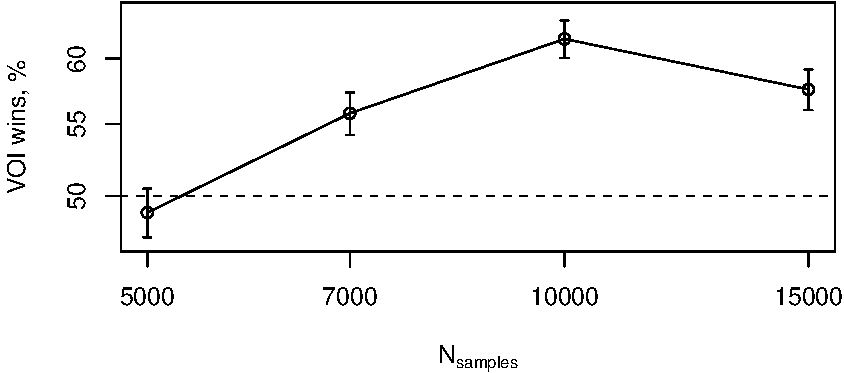
\includegraphics[scale=0.55]{mcts-voi-wins.pdf}
\caption{Winning rate of the VOI-aware policy in Go as a function of the number of samples, fixing cost $c=10^{-6}$.}
\label{fig:voi-wins}
\end{figure}

Figure~\ref{fig:voi-wins}
shows the winning rate of VOI against UCT $c=10^{-6}$. In agreement with the intuition
(Figure~\ref{sec:mcts-control-redistribution}), VOI-based stopping and
sample redistribution is most influential for intermediate numbers of
samples per ply. When the maximum number of samples is too low, early
stopping would result in poorly selected moves. On the other hand,
when the maximum number of samples is sufficiently high, the VOI of
increasing the maximum number of samples in a future state is low.

Note that if we disallowed reuse of samples in both Pachi and
in our VOI-based scheme, the VOI based-scheme
win rate is even higher than shown in Figure~\ref{fig:voi-wins}. This is as expected,
as this setting (which is somewhat unfair to UCT-Pachi) is closer to
meeting the assumptions underlying the selection MDP.

\section{Conclusion and Further Research}

This work suggested a Monte-Carlo sampling policy in which sample
selection is based on upper bounds on the value of
information. Empirical evaluation showed that this policy outperforms
heuristic algorithms for pure exploration in MAB, as well as for MCTS.

MCTS still remains a largely unexplored field of
application of VOI-aware algorithms. More elaborate VOI estimates,
taking into consideration re-use of samples in future search states
should be considered. The policy introduced here differs from
the UCT algorithm only at the first step, where the VOI-aware
decisions are made. Consistent application of principles of rational
metareasoning at all steps of a rollout may further improve the
sampling.

